\chapter{Tensor-RNN: bridge between tensor networks and neural networks}
\label{ch:tensor-rnn}

Comparing tensor network (TN) quantum states in \cref{ch:tn} and neural quantum states (NQS) in \cref{sec:nqs}, we can see that TNs have deeper background in physics, as their representations of the ground states of some important physical systems are found by construction, and their analytical properties such as the entanglement entropy and the spatial correlations are proven. They are also more controllable, in the sense that we can systematically improve the accuracy of variational approximation by increasing their bond dimensions. Their relatively simple multilinear architectures are suitable for second-order optimizations, which have better convergence properties to the ground state than the first-order optimizations usually used for neural networks. However, the 1D matrix product state (MPS) is not expressive enough for 2D and higher-dimensional systems, and the 2D projected entangled-pair state (PEPS) cannot be efficiently contracted.

On the contrary, NQSs are proven to have the expressiveness of universal approximation, and they are practically successful in representing complicated ground states, such as spin liquids, with high accuracy and efficiency. However, their interpretability and controllability are worse than TNs. Their analytical properties, the relation between the accuracy of variational approximation and their hyperparameters, such as the numbers of layers and channels, as well as the optimization methods to fully exploit their expressiveness, are all under research.

Since the initial proposal of NQSs, there has been continuing research on their ability to represent certain classes of quantum states~\cite{gao2017efficient, carleo2018constructing, sharir2022neural}. Exact mappings have been constructed between TNs and NQSs, especially restricted Boltzmann machines (RBM) with relatively simple architectures~\cite{glasser2018neural, chen2018equivalence}. Meanwhile, the mapping from TNs to recurrent neural networks (RNN) has been studied with the concept of recurrent arithmetic circuits~\cite{levine2017long, levine2019quantum}, which suggests that the extra expressiveness of RNNs over TNs can be attributed to their reuse of information between sites.

In the following, we present a series of NQS architectures, namely MPS-RNN and tensor-RNN~\cite{wu2023tensor}, which combine the strengths of TNs and RNNs. They can achieve higher numerical accuracy than MPS and PEPS, show the desired analytical properties of entanglement entropy and spatial correlations, and get systematically improved by increasing the bond dimension, which is the only hyperparameter for their architectures. Moreover, they support exact sampling and efficient evaluation, which lead to reduced practical computational time compared to PEPS.

\section{Vanilla MPS-RNN}

We start from the aforementioned definition of an MPS with bond dimension $\chi$, on $N$ sites of spin-$\frac{1}{2}$ particles:
\begin{equation}
\psi(\vs) = \sum_{a_0, \ldots, a_N = 1}^\chi \prod_{i = 1}^N M^{(i)}_{s_i; a_i, a_{i - 1}}.
\tag{\ref{eq:mps}}
\end{equation}
Note that we use $1$-based indexing for the spatial and the bond dimensions, which is consistent with the notations in previous chapters, as opposed to the $0$-based indexing in Ref.~\cite{wu2023tensor}, which can be more convenient for software implementation. The many-body probability $q(\vs) = |\psi(\vs)|^2$ can be factorized into autoregressive (AR) conditional probabilities~\cite{ferris2012perfect, han2018unsupervised, wei2022sequential}:
\begin{equation}
q(\vs) = \prod_{i = 1}^N q_i(s_i \mid \vs_{< i}),
\tag{\ref{eq:autoreg}}
\end{equation}
which are suitable for exact sampling. Each conditional probability is formally written as:
\begin{align}
q_i(s_i \mid \vs_{< i}) &= \frac
{\vh^{(i) \dagger}(s_i, \vs_{< i}) \mga^{(i)} \vh^{(i)}(s_i, \vs_{< i})}
{\vh^{(i) \dagger}(\vs_{< i}) \mga^{(i)} \vh^{(i)}(\vs_{< i})}, \label{eq:mps-cond-prob} \\
h^{(i)}_{a_i}(\vs_{\le i}) &=
\sum_{a_1, \ldots, a_{i - 1}}
\prod_{j = 1}^i M^{(j)}_{s_j; a_j, a_{j - 1}}, \\
\gamma^{(i)}_{b_i, a_i} &=
\sum_{\substack{a_{i + 1}, \ldots, a_V \\ b_{i + 1}, \ldots, b_V \\ s_{i + 1}, \ldots, s_V}}
\prod_{j = i + 1}^V M^{(j) *}_{s_j; b_j, b_{j - 1}} M^{(j)}_{s_j; a_j, a_{j - 1}},
\end{align}
where $\vh^{(i)}$ is a vector of size $\chi$, denoting the partially contracted sites up to the site $i$, and depending on the spins $\vs_{\le i}$, while $\mga^{(i)}$ is a $\chi \times \chi$ matrix, denoting the partially contracted sites and their conjugates after the site $i$.

\begin{figure}[htb]
\centering
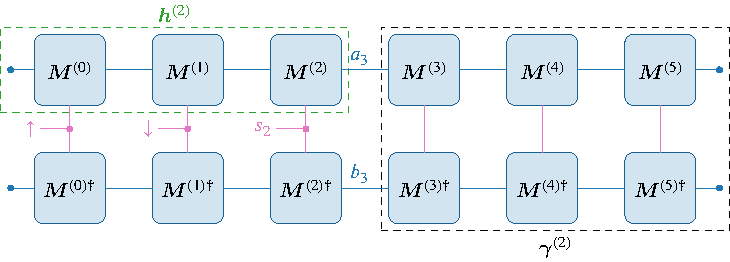
\includegraphics[width=0.8\linewidth]{ch9/mps_cond_prob.pdf}
\caption[Tensor diagram for conditional probability in MPS]{
Tensor diagram for the unnormalized conditional probability $\tilde{q}_3(s_3 \mid s_1 = \spinup, s_2 = \spindown)$ as in \cref{eq:mps-cond-prob}. An MPS with six sites is shown as an example.
This figure is reproduced from Fig.~S1 in the supplemental material of Ref.~\cite{wu2023tensor}.
}
\label{fig:mps-cond-prob}
\end{figure}

The tensor diagram for the numerator of \cref{eq:mps-cond-prob} is shown in \cref{fig:mps-cond-prob}. Note that the solid dot with $r$ indices denotes the rank-$r$ Kronecker tensor
\begin{equation}
\delta_{i_1, \ldots, i_r} = \begin{cases}
1, & i_1 = \cdots = i_r \\
0, & \text{otherwise}
\end{cases},
\end{equation}
and when $r = 1$ it simply sums over the index. As edge cases, we have
\begin{equation}
h^{(0)}_a = 1 \quad \forall a,
\end{equation}
which is just the top leftmost solid dot, and
\begin{equation}
\gamma^{(N)}_{b, a} = 1 \quad \forall a, b,
\end{equation}
which is the direct product of the rightmost two solid dots.

When sampling from $q(\vs)$ in the AR order, we precompute $\mga^{(N - 1)}, \ldots, \mga^{(1)}$ during the usual contraction of $\ip{\psi}$, which are independent of the input spins. Then in each AR sampling step $i$, we update $\vh^{(i)}$ by
\begin{equation}
\vh^{(i)} = \mM^{(i)}_{s_i} \vh^{(i - 1)},
\label{eq:mps-rnn-h}
\end{equation}
which can be interpreted as updating the hidden memory in an RNN, although in the MPS we do not share parameters $\mM^{(i)}$ between different sites $i$. After obtaining $\vh^{(i)}$, we compute the unnormalized probability
\begin{equation}
\tilde{q}_i(s_i \mid \vs_{< i}) = \vh^{(i) \dagger} \mga^{(i)} \vh^{(i)},
\label{eq:mps-rnn-q}
\end{equation}
and normalize it if needed, which can be interpreted as the output layer of the RNN. The tensor diagrams for this AR sampling step are shown in \cref{fig:mps-h-p}.

\begin{figure}[htb]
\centering
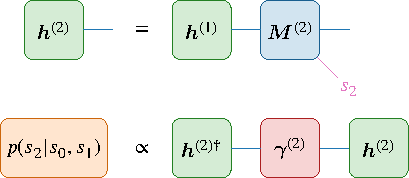
\includegraphics[width=0.5\linewidth]{ch9/mps_h_p.pdf}
\caption[Tensor diagrams for an AR sampling step of MPS]{
Tensor diagrams for updating the memory $\vh^{(i)}$ and computing the conditional probability $q_i(s_i \mid \vs_{< i})$ in an AR sampling step of MPS.
This figure is reproduced from Fig.~1~(b) in Ref.~\cite{wu2023tensor}.
}
\label{fig:mps-h-p}
\end{figure}

Therefore, the MPS is exactly mapped into an RNN architecture with memory size $\chi$, linear updates of the memory in \cref{eq:mps-rnn-h}, and a bilinear output layer in \cref{eq:mps-rnn-q}. We refer to this architecture as the vanilla MPS-RNN. We also mention that besides the probability $q(\vs)$, the complete definition of the wave function includes the phase $\phi(\vs)$:
\begin{equation}
\psi(\vs) = \sqrt{q(\vs)} \rme^{\rmi \phi(\vs)}.
\tag{\ref{eq:psi-q-phi}}
\end{equation}
After the AR sampling of MPS, $\phi(\vs)$ is obtained by
\begin{equation}
\phi(\vs) = \arg \sum_{a} h^{(N)}_a.
\label{eq:mps-rnn-phase}
\end{equation}
The computational graph for the vanilla MPS-RNN to evaluate $\psi(\vs)$ is shown in \cref{fig:rnn-psi}.

\begin{figure}[htb]
\centering
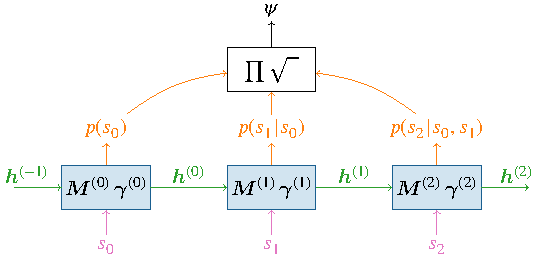
\includegraphics[width=0.7\linewidth]{ch9/rnn_psi.pdf}
\caption[Computational graph for vanilla MPS-RNN]{
This figure is reproduced from Fig.~1~(a) in Ref.~\cite{wu2023tensor}.
}
\label{fig:rnn-psi}
\end{figure}

\section{1D MPS-RNN}

\section{2D MPS-RNN and tensor-RNN}

\begin{figure}[htb]
\centering
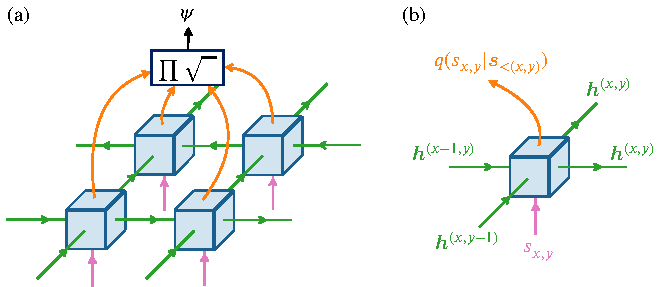
\includegraphics[width=0.8\linewidth]{ch9/tensor_rnn_all.pdf}
\caption[Computational graph for tensor-RNN]{
This figure is reproduced from Fig.~2 in Ref.~\cite{wu2023tensor}.
}
\label{fig:tensor-rnn-all}
\end{figure}

\begin{figure}[htb]
\centering
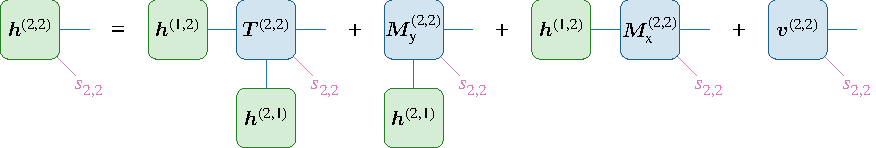
\includegraphics[width=\linewidth]{ch9/tensor_rnn_h.pdf}
\caption[Tensor diagram for memory update of tensor-RNN]{
This figure is reproduced from Fig.~3 in Ref.~\cite{wu2023tensor}.
}
\label{fig:tensor-rnn-h}
\end{figure}

Another architecture~\cite{hibat2021variational, hibat2022supplementing}

Mixture of neural and tensorial layers~\cite{chen2023antn}

\section{Numerical results}

\begin{figure}[htb]
\centering
\hspace*{-0.05\linewidth}
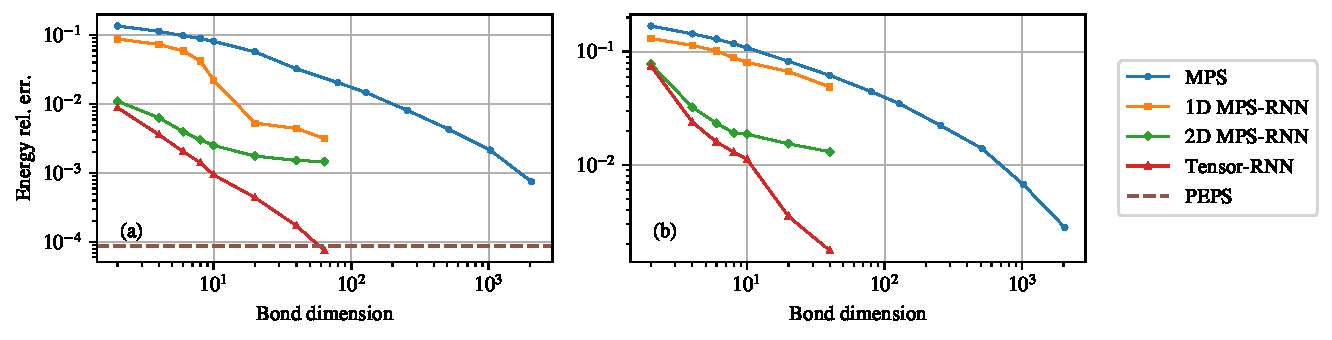
\includegraphics[width=1.1\linewidth]{ch9/tensor_rnn_energy_chi.pdf}
\caption[Variational energy vs. bond dimension for tensor-RNN]{
This figure is reproduced from Fig.~4 in Ref.~\cite{wu2023tensor}.
}
\label{fig:tensor-rnn-energy-chi}
\end{figure}

\begin{figure}[htb]
\centering
\hspace*{-0.05\linewidth}
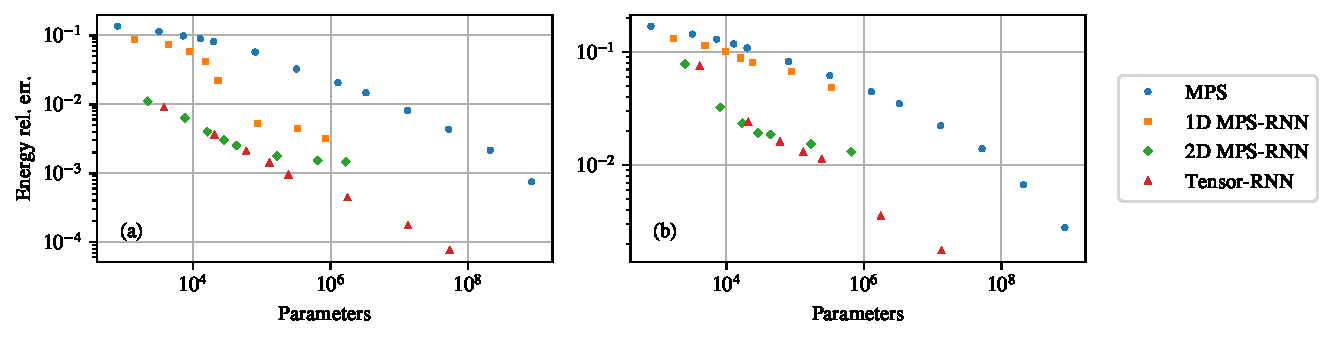
\includegraphics[width=1.1\linewidth]{ch9/tensor_rnn_energy_param.pdf}
\caption[Variational energy vs. number of parameters for tensor-RNN]{
This figure is reproduced from Fig.~S3 in the supplemental material of Ref.~\cite{wu2023tensor}.
}
\label{fig:tensor-rnn-energy-param}
\end{figure}

\begin{figure}[htb]
\centering
\hspace*{-0.05\linewidth}
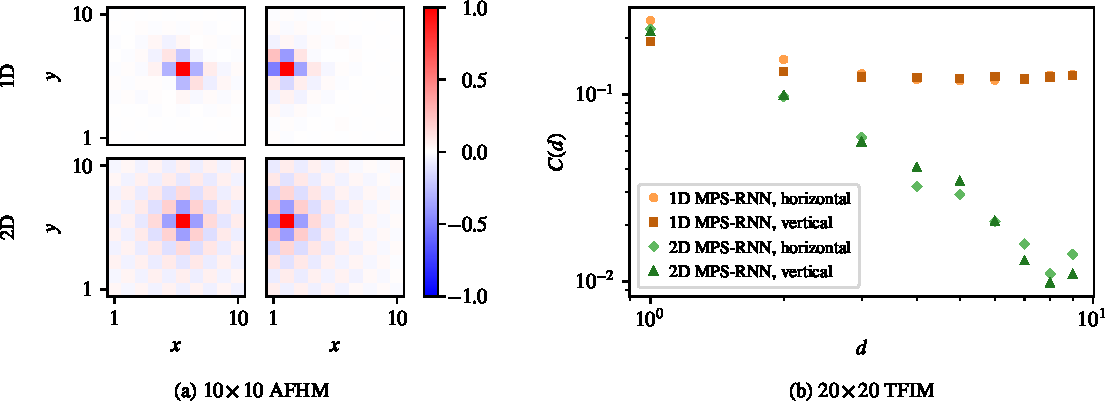
\includegraphics[width=1.05\linewidth]{ch9/tensor_rnn_corr.pdf}
\caption[Spin correlations in MPS-RNN]{
This figure is reproduced from Fig.~S4 in the supplemental material of Ref.~\cite{wu2023tensor}.
}
\label{fig:tensor-rnn-corr}
\end{figure}

\begin{figure}[htb]
\centering
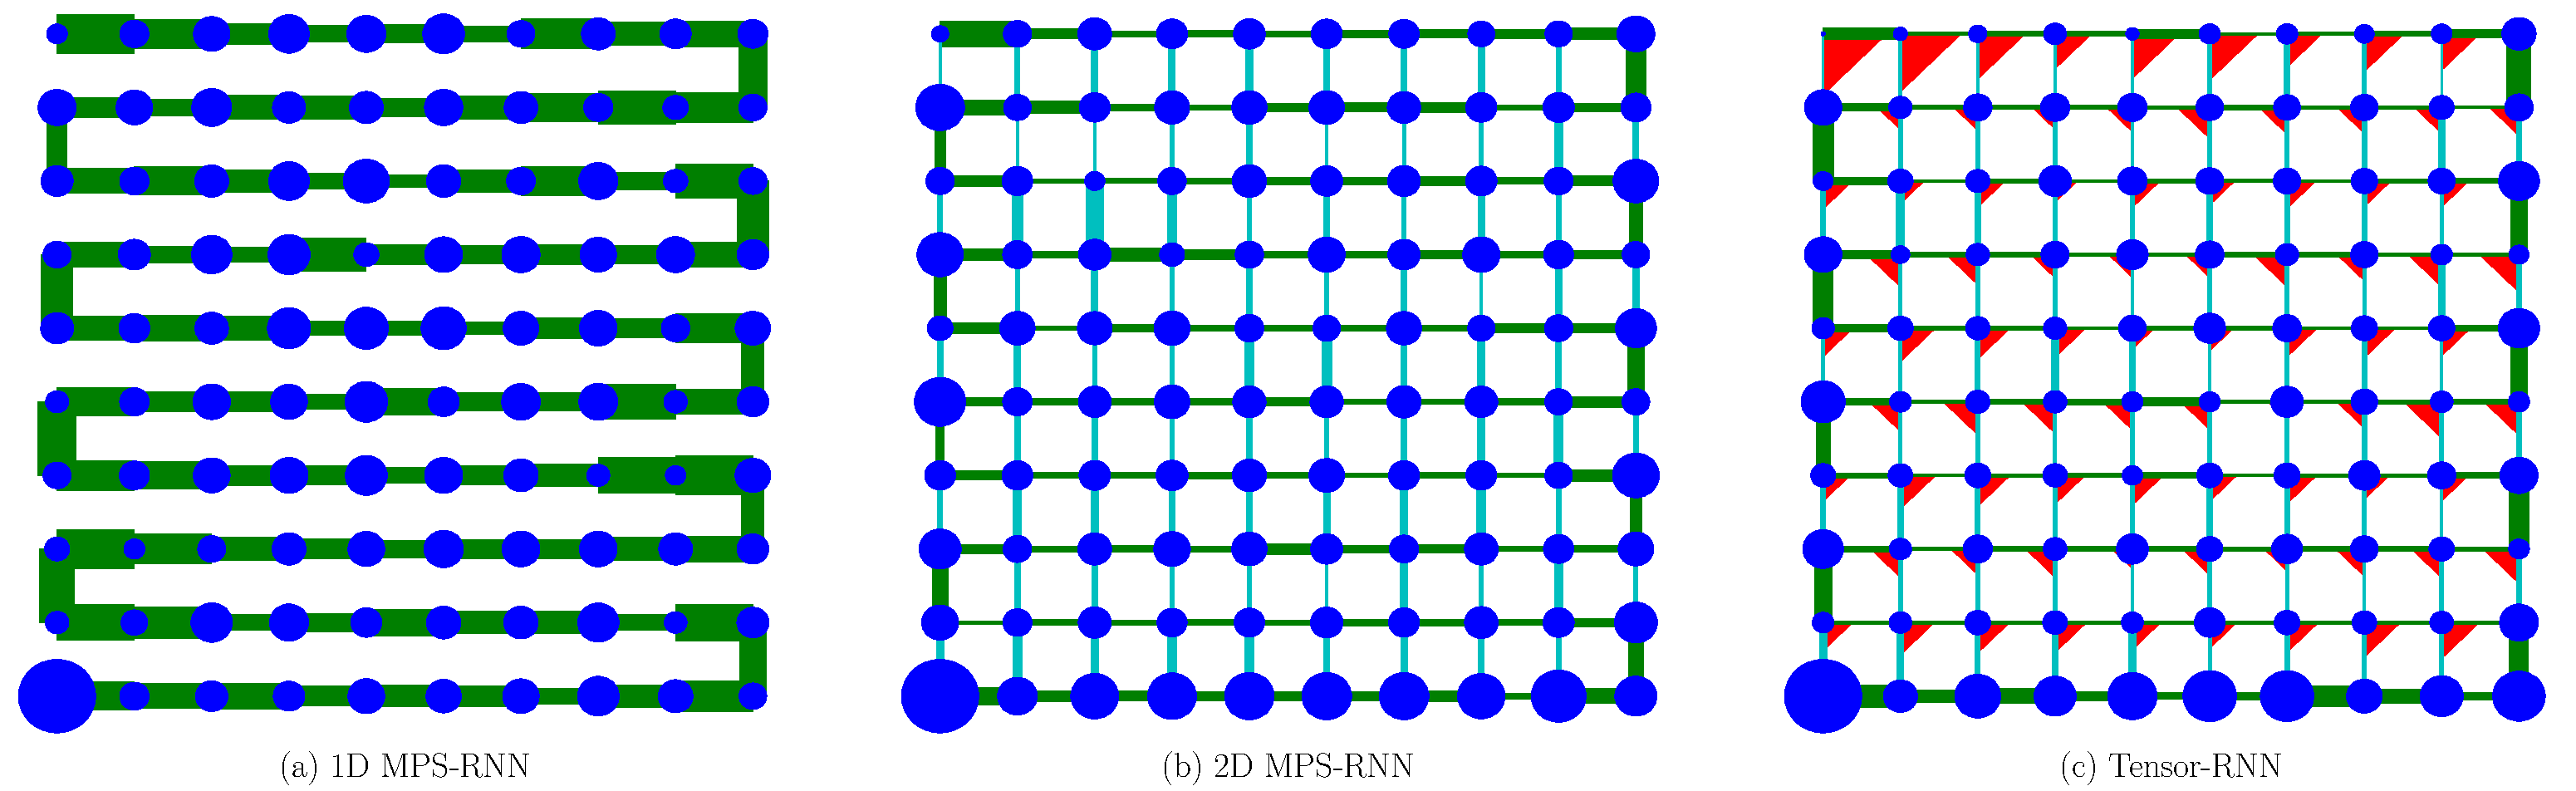
\includegraphics[width=\linewidth]{ch9/tensor_rnn_h_comp.pdf}
\caption[Magnitudes of tensor, matrix, and vector terms in tensor-RNN]{
This figure is reproduced from Fig.~S5 in the supplemental material of Ref.~\cite{wu2023tensor}.
}
\label{fig:tensor-rnn-h-comp}
\end{figure}

\chapter{VarBench: variational benchmarks for quantum many-body systems}
\label{ch:varbench}
